\documentclass{letter}
\usepackage{graphicx}

\begin{document}

Dear Editor,\\

We have substantially revised the manuscript, which we believe is now suitable for publication.

Reviewer 1 argued that the presented models 'did not result in any significant advance in the forecast of Dst index'. We have deliberately avoided to present a direct comparison with other published methods. Although that should be the standard way to present and corroborate new models, we have been discouraged to do so, for a number of reasons. Any such direct comparison can always be debated when some codes are not publicly available. For instance, the code for the celebrated NARMAX model by the Sheffield group is kept secret. Hence, trying to reproduce their model is a very error-prone exercise. Instead, we have decided to make all our codes available. Moreover, we feel that well established standard metrics on which to evaluate the performance of models are still missing in this community.

Finally, a major reason to avoid such comparison is that we agree with Referee 2, that the one-hour ahead is of little practical use, because of its strong persistence behavior. Nevertheless, by introducing a new methodology, this manuscript represents an important step towards the formulation of multiple hour ahead predictions, which is our next goal.\\

In any case, for your eyes only we include here a figure showing the comparison of our models with other published models. Our model outperforms all of them.

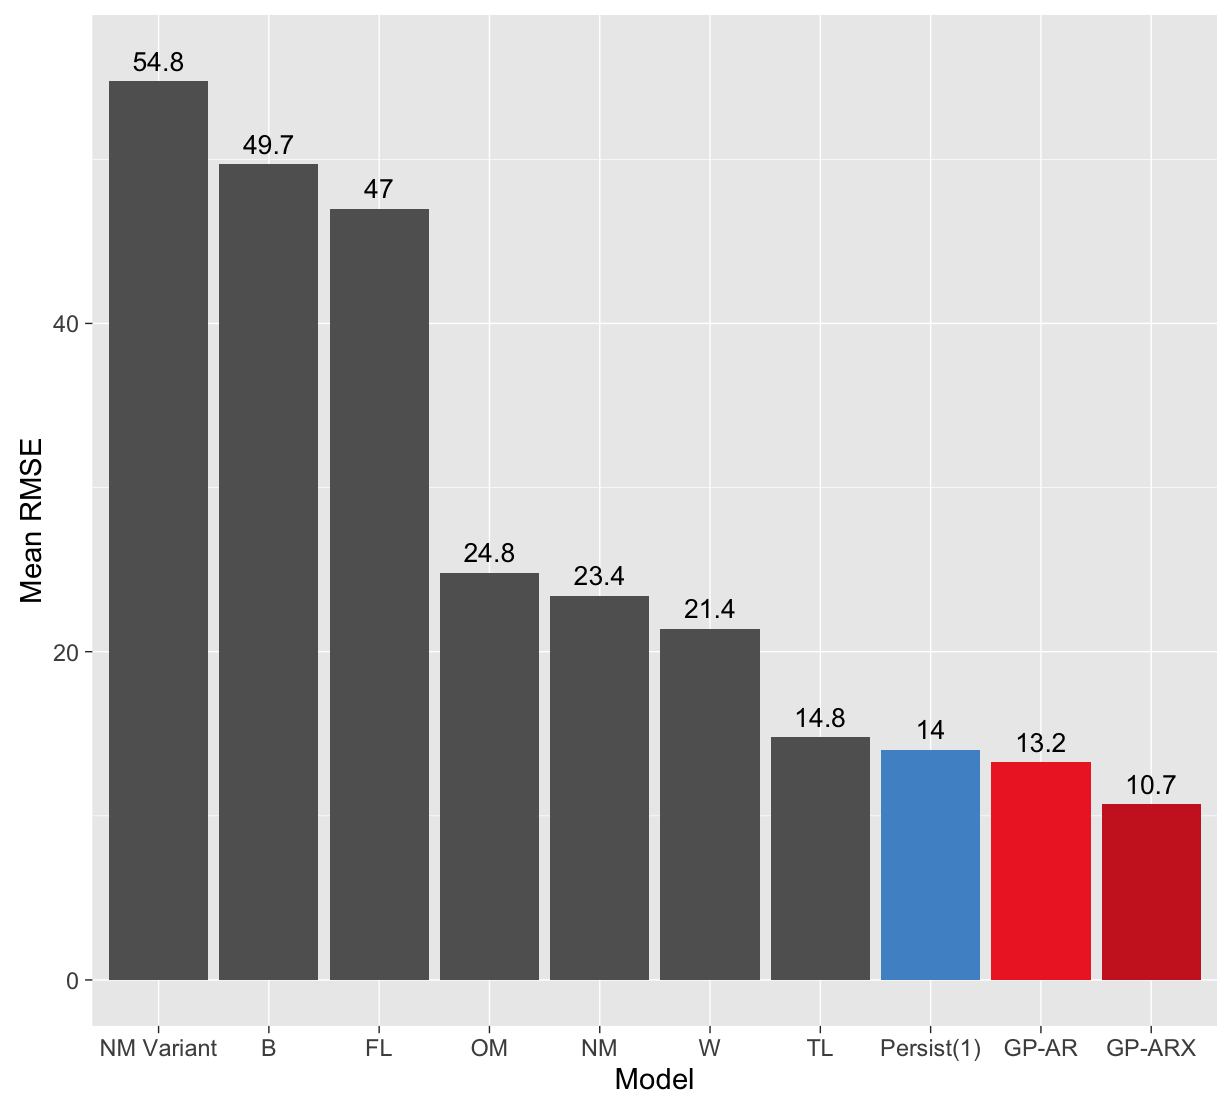
\includegraphics[width=\textwidth]{figures/Compare_RMSE.png}

Regarding reviewer 2, we have done our best to address his/her concerns. However, we would like to point out that the meaning of some comments was rather obscure, due to his/her poor English.

Best regards,
The authors.

\hfill



\end{document}